 \startchapter{Background and Related Work}
\label{chapter:problem}
\newlength{\savedunitlength}
\setlength{\unitlength}{2em}


Computational Linguistics is a field which focuses on understanding the various process through which humans learn, represent, and interpret languages. The lessons learned from such studies could help us to engineer various AI models which could then be used to mimic humans at various tasks. For example, the study of semantic and syntactic properties of language using large text corpora has helped us to develop better speech to text and machine translation systems. The study of semantic properties of images has enabled us to build computational models which have surpassed the average humans capabilities at the task of object recognition from images. Researchers have also studied language representation in human brain through brain imaging technologies such as fMRI, MEG, EEG etc. 

Researchers in the field of psycholinguistics have tried to isolate regions in the brain corresponding to the processing of language. These studies could help us develop better medical techniques to help people suffering from language deficiencies such as Alzheimer’s disease, severe brain damage, Semantic Dementia etc. The language representations in the brain are often studied by comparing neural activations extracted using brain imaging technologies with language models derived from images and text. Brain, images and text could be considered as different representations of language and are modeling the same world phenomenon. For example, reading or seeing an image of a concept such as \textit{cat} brings about the same response in us human beings.

This thesis mainly focuses on the study of similarities between semantic models build from brain, text and images sources. To summarize, this chapter will focus on various related work in the below areas,

\begin{enumerate}
\item The study of semantics in the human brain with the help of semantic models build from text corpora.
\item Methods to evaluate Distributed Semantic models build from text corpora.
\item Study of semantics in images.   
\item Convolutional Neural Networks (CNN) and need to visualize and understand these networks.
\item Existing techniques developed to visualize and understand CNN models and its limitations.
\end{enumerate}

\section{Learning Semantics in Brain}
%Good to talk about understanding language acquisition.
% Talk about understanding language deficiencies in people with learning disabilities

Language acquisition is considered as an important human trait, and the study of the human brain could help us to gain knowledge about how language is decoded and interpreted by us. The development of brain imaging technologies such as Functional Magnetic Resonance Imaging (fMRI), Electro-Encephalogram (EEG), Magnetoencephalography (MEG) has helped Linguists studying semantic decoding in the human brain. Semantic models build from text-based corpora are often used as ground truth to study neural activations related semantic decoding in the brain. The primary reason for such adoption is that corpus-based models are easier to construct and use in the experiments as compared to models build on brain imaging data or images.

Brain imaging technologies such as fMRI, EEG, and MEG are expensive, and construction of semantic models based on these techniques is not feasible. Moreover, the time required to collect enough brain data to build semantic models is extensive. It is not feasible to construct models based on images either since collection and storage of large database of images is not an easy task. The extraction of semantic features from images are computationally expensive. These reasons could explain why distributional semantic models based on the text are widely adopted by researchers to study other representations of language.

The use of semantic models derived from textual data to study neural activations in the brain began with the work of  Mitchell et al. (2008)~\cite{Mitchell1191}. In their experiments, nine right-handed participants were presented with line drawings, and noun labels of 60 concrete nouns on a screen and the neural patterns of the participants were recorded using fMRI. Semantic features corresponding to 25 verbs based on their co-occurrence with each other were then extracted from a large text corpus. Subsequently, a computational model was then trained to predict the neural activity corresponding to unseen concepts.

Murphy et al. (2009) showed that text-based language models could predict EEG activity related to semantics in the brain~\cite{MurphyEEG}.  This was followed by Sudre et al. (2012) who performed similar work using MEG data collected from subjects viewing images of 60 concrete nouns \cite{SUDRE2012451}. Anderson et al. (2015) found that text-based distributional semantic models are better at predicting conceptual similarity in fMRI brain scans of areas linked with linguistic processing, whereas semantic features extracted from images are better at accounting for similarity in visual processing areas in the human brain~\cite{andersonBrainEyes}. In short, semantic similarity based on co-occurrence of words in text corpora could be used to study semantic representations in the human brain.

\section{Learning Semantics in Text}

In the previous section, we discussed various techniques that are adopted by the Computational Linguistics community to study semantic representation in the human brain. We also discussed in brief about Distributional Semantic (DS) models or word vectors extracted from text-based corpora which are used as ground truth to predict activity related to semantics in the brain. In this section, we discuss some of the most popular word vector models that are available today. These models are extensively used in various NLP related tasks such as sentiment analysis, document classification, machine translation etc. The main idea behind word vectors is that
meaning of a word can be inferred from contextual information.

People learn the meaning of words that they have never seen before by guessing the meaning of
the new word from its context (by understanding the meaning
of the known nearby words). In linguistics, we explain this
in terms of word co-occurrence which is often associated with
semantic proximity and is the principle idea behind the creation of most of present-day DS models or word vectors.

The idea of representing semantic information of a word using
vectors is not new and could be traced back to Charles
Osgood’s work \textit{Semantic Differentials} in 1965~\cite{osgood1965cross}. In his work,
Osgood used handcrafted methods to build feature
representations to study semantic similarities between words. In a hand-crafted lexical source, the relationship between words is assigned by human annotated based on a set rule. In the early 2000s, the use of neural networks to generate word vector representations became popular among the linguistics community. In
2003, Bengio et al. trained a probabilistic neural network model to learn the joint probabilistic distribution of
sequences of words in a language~\cite{bengio2003neural}. Collobert and Weston, 2008 were perhaps the first to successfully demonstrate that neural network
architecture could be used to learn word vectors
representing semantic information from a text corpus~\cite{collobert2008unified}. They
experimentally argued that word vectors learned from a large text corpus could be used as an effective tool to perform various downstream tasks
in NLP. 

Mikolov et al. introduced the \textbf{Word2Vec} model in 2013 and triggered
a revolution in the field of NLP~\cite{Word2Vec}. The
Word2Vec model was released as a toolkit which made it easier to train new word vectors from a text corpus which culminated in their rapid adoption by the industry.  Word2Vec uses a shallow two-layer neural network architecture to learn the semantic features from the text. The input to the network is a one-hot sparse vector representing a word and output layer is a probabilistic layer which predicts probabilities of various words in the vocabulary given the input word. This simple neural network is trained to perform a task such as to predict words used in context of a given word. After the network is fully trained, the weights corresponding to the hidden layers for a given input word is extracted as its word vector. The dimensions of the word vector is equivalent to the number of neurons in the hidden layer of the neural network. Word2Vec model consists of two distinct algorithms, a continuous bag
of words (CBOW) and Skip-gram model. 

\begin{description}
\item[$\bullet$]A CBOW model was
trained to predict a target word given a set of words
surrounding it. In vector space, this can be visualized as
predicting the distance between two different word vectors
which are in context to one another.
\item[$\bullet$]  For Skip-gram, the
direction of prediction is reversed, i.e., from a source word it tries to predict all the words which are in context to the source word. The Skip-gram model trained on Google
news dataset is a 300-dimensional vector.
\end{description}



\textbf{Glove} is a regression-based semantic model published by Pennington et al. in 2014 \cite{Glove}. It introduces the concept of representing the relationship between two word as their co-occurrence probabilities. This 300-dimensional vector model was trained on a combined corpus of Wikipedia and Gigaword 5~\cite{graff2003english}.

\textbf{Global Context} is another DS model that takes into account both local, and global context of a document to learn the semantics of the word (Huang et al., 2012)~\cite{GlobalContext}. This model could  encode into the word vectors properties such as homonymy and polysemy of a word. Homonymy refers to the relationship between words with identical forms, but different meanings. Oxford dictionary defines polysemy as \textit{``the coexistence of many possible meanings for a
word or phrase''}~\cite{simpson1989oxford}. 

\textbf{Cross-lingual} is a model proposed by Faruqui
and Dyer, 2014, takes into account semantic properties across various languages \cite{Crosslingual}. It was trained using both German and English words using WMT-2011 corpus and uses a shared semantic space to learn the word embeddings.

\textbf{RNN} model is based on a  Recurrent Neural Network (RNN) that is trained to predict the next word in the sequence (Mikolov et
al., 2011) \cite{RNN}. Unlike Skip-gram and other models which derives word vectors from an n-gram of words (Three or four words which occur together), a RNN model can theoretically
represent words at infinite distance from one another. This model trained on broadcast news transcriptions has a dimension of 640 for its word embeddings. 

A Recurrent Neural Network is a type of Artificial Neural Network designed to model  sequential information. A RNN considers inputs not only in the current time step but also the inputs from previous time steps to perform various network operations. Compared to other neural models, RNNs pass their hidden state across invocations which functions as a memory through the previous time steps. This network is mostly used as a generative model.


\textbf{Non-Distributional} is another semantic word vector model created
by combining various hand-crafted lexical sources such as
WordNet (Fellbaum,1998)~\cite{wordnet}, FrameNet (Baker,1998)~\cite{FrameNet}, Emotion \&
Sentiment (Mohammad and Turney,2013)~\cite{mohammad2013crowdsourcing} etc. by Faruqui et al.~\cite{NonDist}. In a hand-crafted lexical source, the relationship between words is assigned by human annotated based on a set rule. For example in WordNet, the words are arranged in a hierarchical manner based on their meaning. Word vectors produced by this model are highly sparse, and each dimension of a vector in this model could be traced back to a linguistic feature. An example of a linguistic feature would be emotions which are triggered by a concept (positive, negative, fear, anger etc.). Another example would be part of speech features such as noun, proverb, adjective etc.

%Why they are called Distributed models of semantics

The various word vector models described in this section are also referred to as \textit{Distributed models of Semantics} (DS) because the semantic information of a word is distributed throughout the dimensions of the vector.  Due to their widespread adoption into various NLP tasks, it becomes important to evaluate and benchmark these word vector models.


%%%%%%%%%%%%%%%%%%%%%%%%%%%%%%%%%%%%%%%%%%%%%%%%%%%%%%%%%%%%

\section{Evaluation of Word Vectors}
Traditionally computational linguistic community has relied on word similarity tasks to evaluate and benchmark various word vectors. These methods are based on computing the distance between word vectors and some similarity measure assigned by human annotators for the same word pairs. Some popular word similarity tasks used to evaluate word vectors are discussed below:

\subsubsection{MEN} A dataset that consists of 3000-word similarity pairs with human-assigned similarity judgments collected using Amazon Mechanical Turks (AMT)~\cite{MEN}. The words that occur at least 700 times from the \textit{ukWaC}~\cite{ukWaC} and \textit{Wackypedia}~\cite{WaCky} corpora were included in this dataset. The human annotators were presented with a pair of words and asked to assign a similarity score in a standard 1-7 Likert scale.

\subsubsection{WS-353} This dataset contains 353-word pairs assigned similarity scores by human annotators~\cite{WS-353}. Agirre et al., 2009 claimed that similarity and relatedness denote different relationships among words. Based on this argument, the WS-353 dataset was further split into WS-SIM and WS-REL with each set containing 353 pairs of words~\cite{agirre2009study}.

\subsubsection{SimLex-999}

SimLex-999 dataset focuses on measuring similarity in semantic models rather than relatedness or association between words~\cite{hill2015simlex}.  SimLex-999 has word pairs with varying degree of concreteness. The whole dataset is further divided into 666 noun-noun pairs, 222 verb-verb pairs and 111 adjective-adjective pairs.



\subsubsection{Evaluating Word vectors Using Brain Data}

The evaluation of word vectors using word similarity datasets are quite popular and widely accepted by the research community. However, Faruqui et al., 2016 highlighted some serious limitations with the use similarity datasets to benchmark and compare word vectors~\cite{W16-2506}. Most of the Distributed models for semantics are task specific and not entirely trained to capture word co-occurrence. Moreover, similarity datasets do not capture the notion of polysemy and therefore penalizes word vectors which take into account of polysemy in words. The current evaluation techniques also fail to take into consideration of statistical significance when measuring the difference in the performance of two word vectors models on a similarity dataset. Based on their observations, Faruqui et al. concluded that more research into methods to evaluate word vectors were necessary.

In 2016, Xu et al. introduced \textit{BrainBench}: a system designed to test text-based Distributed Semantic models using brain data \cite{BrainBench2016}. As discussed in chapter \ref{chapter:introduction}, the first iteration of BrainBench was based on two brain image datasets: a fMRI dataset \cite{Mitchell1191} and a MEG dataset \cite{SUDRE2012451} collected from nine participants. They tested six popular word vector models against the fMRI and MEG datasets and the results are summarized by the Figure:~\ref{BrainBench11}). In this thesis, we release the second iteration of BrainBench which is described in detail in the chapter \ref{chapter:newsol} of this thesis.

\begin{figure}[t]
\begin{tabular}{ll}
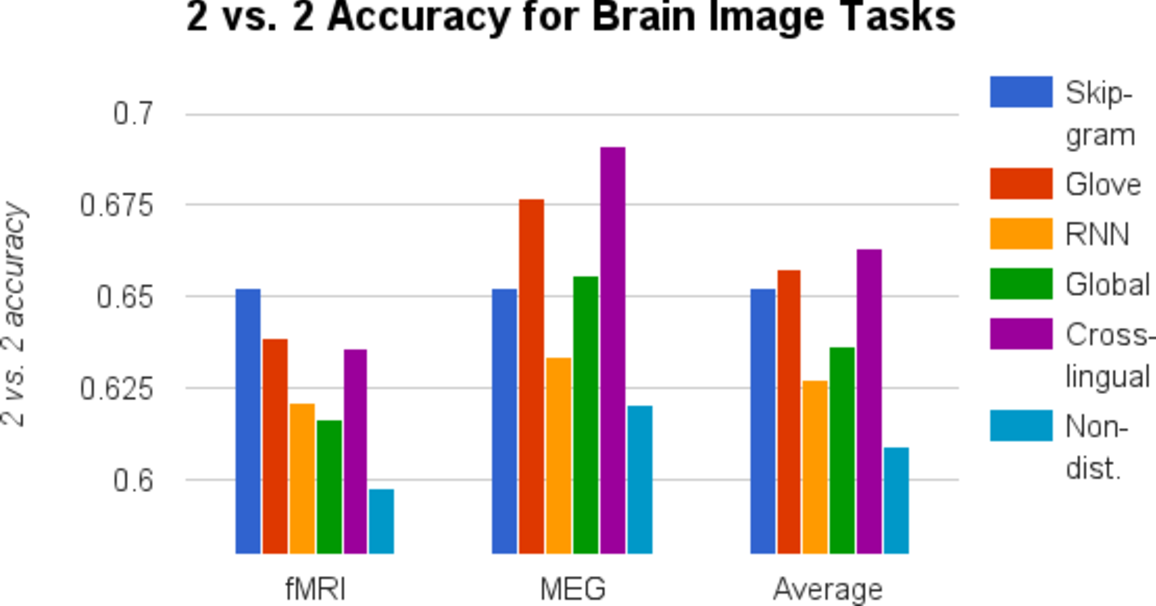
\includegraphics[width =7cm,height=4cm]{Figures/brainbench}
&
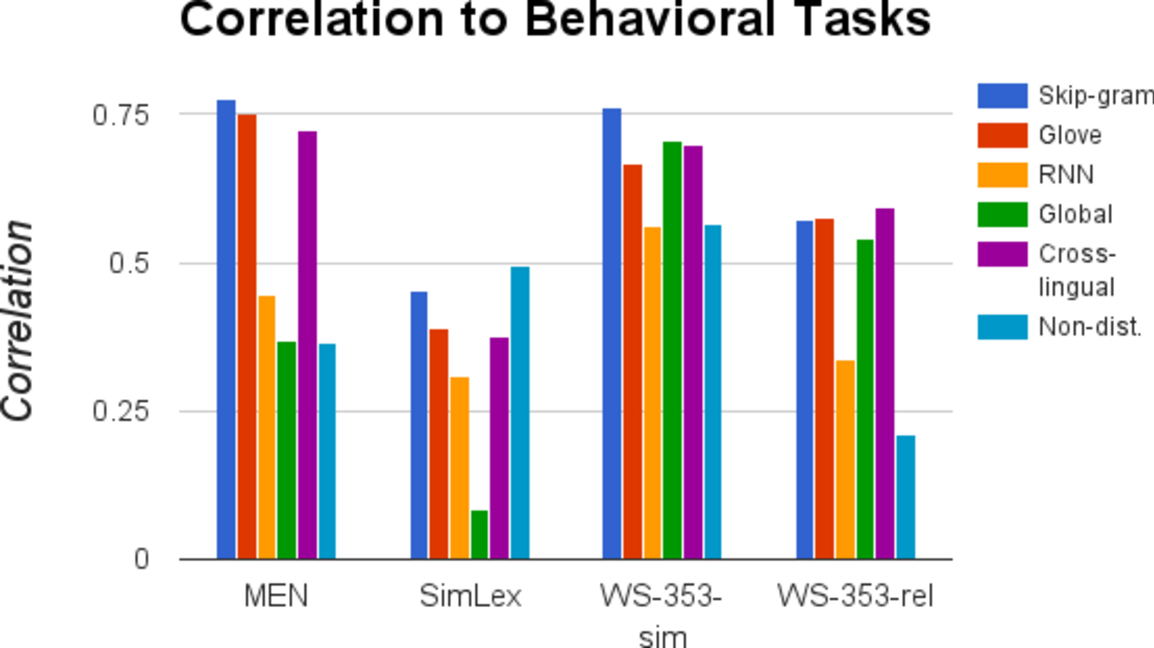
\includegraphics[width =7cm,height=4cm]{Figures/brainbench2}
\end{tabular}
\caption{Comparison of BrainBench Performance against other word Similarity dataset}
\label{BrainBench11}
Left shows the BrainBench test results for 6 popular DS models and Right shows the comparative performance of the same DS models on other word similarity tasks. Image source: Xu et al.,2016~\cite{BrainBench2016}.
\end{figure}


\section{Learning Semantics from Images}

The beginning of 21st century witnessed tremendous development in the field of digital camera technology which resulted in the explosion of high resolutions images on the Internet. Image search and retrieval tasks on the Internet required the images to be annotated with semantic keywords labels. However, the volume of pictures uploaded to the Internet grew exponentially since the year 2000 and Labeling these images manually using human annotators were costly and time-consuming. Moreover, such methods had a high degree of annotation inaccuracy due to the subjectivity
of human perception. Therefore it became imperative to develop techniques to label these images into semantic categories automatically.

A popular technique introduced by researchers in computer vision is content-based image retrieval
(CBIR). In this method, the images were indexed by low-level visual features such as color,
texture, shapes. The low-level features such as color, texture, shape etc. are extracted from images using techniques such as HOG, SIFT etc. from whole or segmented regions of an image. Once these low-level features are extracted, supervised machine learning models such as Support Vector Machines (SVM)~\cite{feng2003bootstrapping}, Decision Trees~\cite{shyu2000relevance} and Bayesian classifiers~\cite{jin2004semi} were trained on these low-level features to learn high-level concepts from images. However, these supervised models still required the images to be manually annotated before they could be trained on extracted features. The use of unsupervised machine learning models such as k-means clustering was also popular in CBIR systems. 

Most of state of the art systems in computer vision used today are based on neural networks. Unlike classical text-based and context based image retrieval techniques, neural networks learn features automatically from images. The origin of these computational models could be traced back to early 1970's and mimics the perceptual system in mammals.

The human visual cortex helps us to interpret the visual stimulus and derive semantics from our sight. In 1962, Hubel and Wiesel studied the perceptual system in cats and concluded that the visual cortex in the brain is made up of special arrangements of cells which are sensitive to only specific regions in the visual field \cite{Hubel992}. These cells or neurons only fire in the presence of edges of certain orientations or patches of colour. They act as local filters and are tiled across the entire field of view. They also identified other complex cells which have a much larger receptive field and takes input from the cells which act as local filters. They, in turn, are connected to other cells with an even larger receptive field. This results in a columnar arrangement of cells and results in visual perception. The semantic representation in images could be studied with the help of Convolutional Neural Networks (CNN).


Convolutional Neural Networks is a type of Artificial Neural Networks (ANN) loosely inspired by the human visual cortex.  They are quite popular among the computer vision community and are used for image recognition. Just like the brain, they also contain neurons (perceptron) which work together to form filters. These filters are slid across the entire image, and this results in feature maps. This sliding operation is commonly referred to as convolution. The first layer of any CNN is a convolutional block which takes an image as input. The neurons in the beginning layers of a CNN learn low-level features such as edges, orientation, colour patches etc. These low-level features learned by the initial layers are given as input to latter layers which learns high-level feature representations. Based on these high-level features, a CNN can identify and label objects correctly~\cite{CNNREF1, CNNREF2}.




Prior to Convolutional Neural Networks, classical computer vision techniques such as the Naive Bayes classifier using a bag of visual features \cite{Csurka2004}, hierarchical Bayesian models for object categorization \cite{SivicREZF05} and many others were used for object recognition. These methods required a lot of preprocessing and extraction of handcrafted features such as Histogram of Oriented Gradients (HOG) or Scale-invariant Feature Transform (SIFT) from the images before they could be trained to predict images. However, in CNNs the features are learned automatically by the filters, and the input image requires very little pre-processing. CNNs also outperformed other classical methods in various image recognition tasks which led to their rapid adoption by researchers and industry. 


\subsection{A brief history of Convolutional Neural Networks}
\textit{Neocognitron}, the first CNN developed in 1982 by  Kunihiko Fukushima used a hierarchical multiple layer architecture \cite{FukushimaM82}.  The Neocognitron could recognize various patterns in images based on the difference in their shapes. This was followed by LeNet architecture developed by Yann LeCun of Bell labs who demonstrated that Convolutional Neural Networks could be used for recognition of handwritten digits \cite{LeNet1989}. The development of faster computers and Graphical Processing Units (GPU) created a revolution in the field of CNNs.  A major limitation of CNN is that it requires a large number of labelled images to learn from various patterns in images and make successful predictions. 


In 2009, Fei-Fei et al. released \textit{ImageNet} - a free database of 14 million images of 1000 categories, collected and labeled using the Internet \cite{ImageNet2009}. This lead to the genesis of ImageNet Large Scale Visual Recognition Competition (ILSVRC)-  a benchmark competition for object category classification from images \cite{ImageNETChallenge}. Equipped with the processing power of GPU and labeled training images from ImageNet, Krizhevsky et al. released AlexNetwhich achieved a top 5 test error rate of 15.4\% in the ILSVRC, 2012 competition becoming state of the art in the field of object recognition \cite{Alexnet2012}. A top 5 error is defined as the rate at which the model does not predict the correct label in its top 5 predictions. It may be worth noting that the second place entry in the competition was a non-CNN variant that had a top-5 error rate of 26.2\%. 

The success of AlexNet caught the attention of the computer-vision community, and Convolutional Neural Networks started gaining popularity. AlexNet had an eight-layer architecture and one of the deepest network created at that time. Zeiler and Fergus made small modifications to the AlexNet by reducing the stride and filter size of the first layer of AlexNet and performed an extensive hyper-parameter search during training. This modified network dubbed as ZFNet won the  ILSVRC, 2013 competition with a top-5 error of 14.8\%~\cite{ZFNET}. The success of AlexNet and ZFNet set the trend among the research community that having a large number of convolutional blocks and hidden layers in the architecture could somehow improve performance. In short, to get better performance, you need to have a deeper architecture with more convolutional layers. The term \textit{deep learning} was coined to represent the creation and study of such large neural networks.


\begin{figure}[t]
\centering
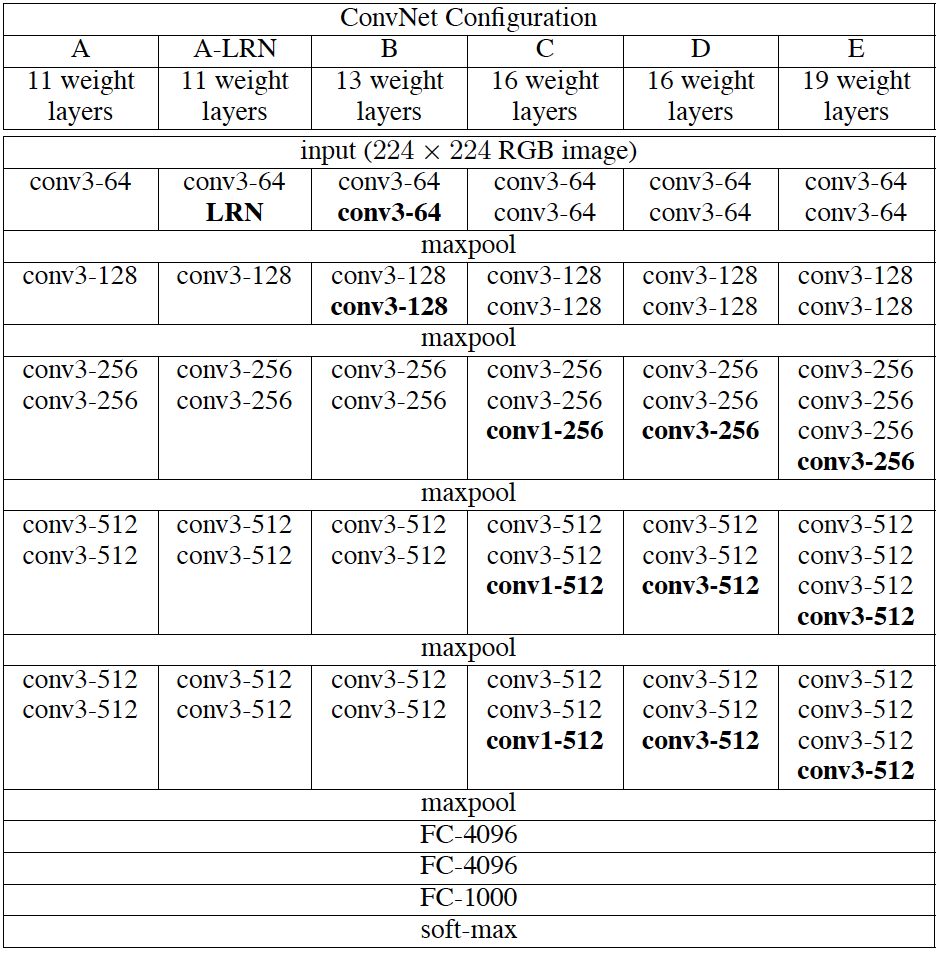
\includegraphics[width=12cm, height=12cm]{Figures/VGG16_Network}
\caption{Variants of the VGGNet architecture}
\label{VGG16_types}
This table shows the different variants of the VGGNet architecture. The configuration D (VGG16) produced the best results in the ILSVRC, 2014 competition in the task of object classification. We use the VGG16 variant for our experiments. Image source: Zisserman and Simonyan.,2014~\cite{VGG16}.
\end{figure}


\subsubsection{The VGGNet Architecture}
ILSVRC, 2014 competition showcased further improvements in the development of the CNN architecture and image recognition. Two notable entries into this competition were the VGGNet and GoogLeNet. The VGGNet architecture designed by Zisserman and Simonyan of the Oxford University was the runner-up for the ILSVRC, 2014 competition in the object recognition category~\cite{VGG16}. The VGGNet have six different architecture variants as shown in Figure:~\ref{VGG16_types} and the configuration D produced the best results in the competition with a top-5 error rate of 7.3\%. This network referred to as VGG16 has 16 layers (13 Convolutional layers and 3 fully connected layers) with over 138 million parameters. It has a homogeneous architecture and performs only 3*3 convolutions and 2*2 max-pooling throughout the architecture. Another important observation from Figure:~\ref{VGG16_types} is that the number of filters doubles after each max-pooling layer which instill the notion of growing depth while shrinking dimensions of the features.


The VGGNet was among the first few CNN architectures which showed that depth of the network was a necessary component for achieving good performance in object recognition tasks. This network is also the preferred network among the computer vision community for extracting features from the images and its weights pre-trained on ImageNet are readily available for download. 
\subsubsection{The Inception architecture}
 The GoogLeNet introduced by Szegedy et al.  was the winner of the ILSVRC 2014 competition at the task of object recognition with a top-5 error of 6.7\%~\cite{GoogleNet} on the ImageNet cross-validation dataset. The main contribution of this network was the introduction of the \textbf{inception module} which drastically reduced the number of parameters in the network without loss in performance.

Before the introduction of GoogLeNet, other states of the art networks such as AlexNet~\cite{Alexnet2012}, VGGNet~\cite{VGG16}, and ZF Net~\cite{ZFNET} etc. had a sequential structure formed by stacking convolutional layers, pooling and fully connected layers on top of each other. However, the inception modules have network operations ($1*1$, $3*3$ and $5*5$ convolutions, max-pooling etc.) happening in parallel as shown in Figure:~\ref{InceptionModules}. The use of different filter patches with different strides helps in multi-level feature extraction and gives the option of varying receptive fields.  The authors also argued that since pooling layers are an important component in state of the art CNNs, adding a max-pooling layer in parallel to the convolution operations could provide a boost in performance. The pooling layers help to reduces spatial sizes and helps to prevent over-fitting.   

\begin{figure}[t]
\centering
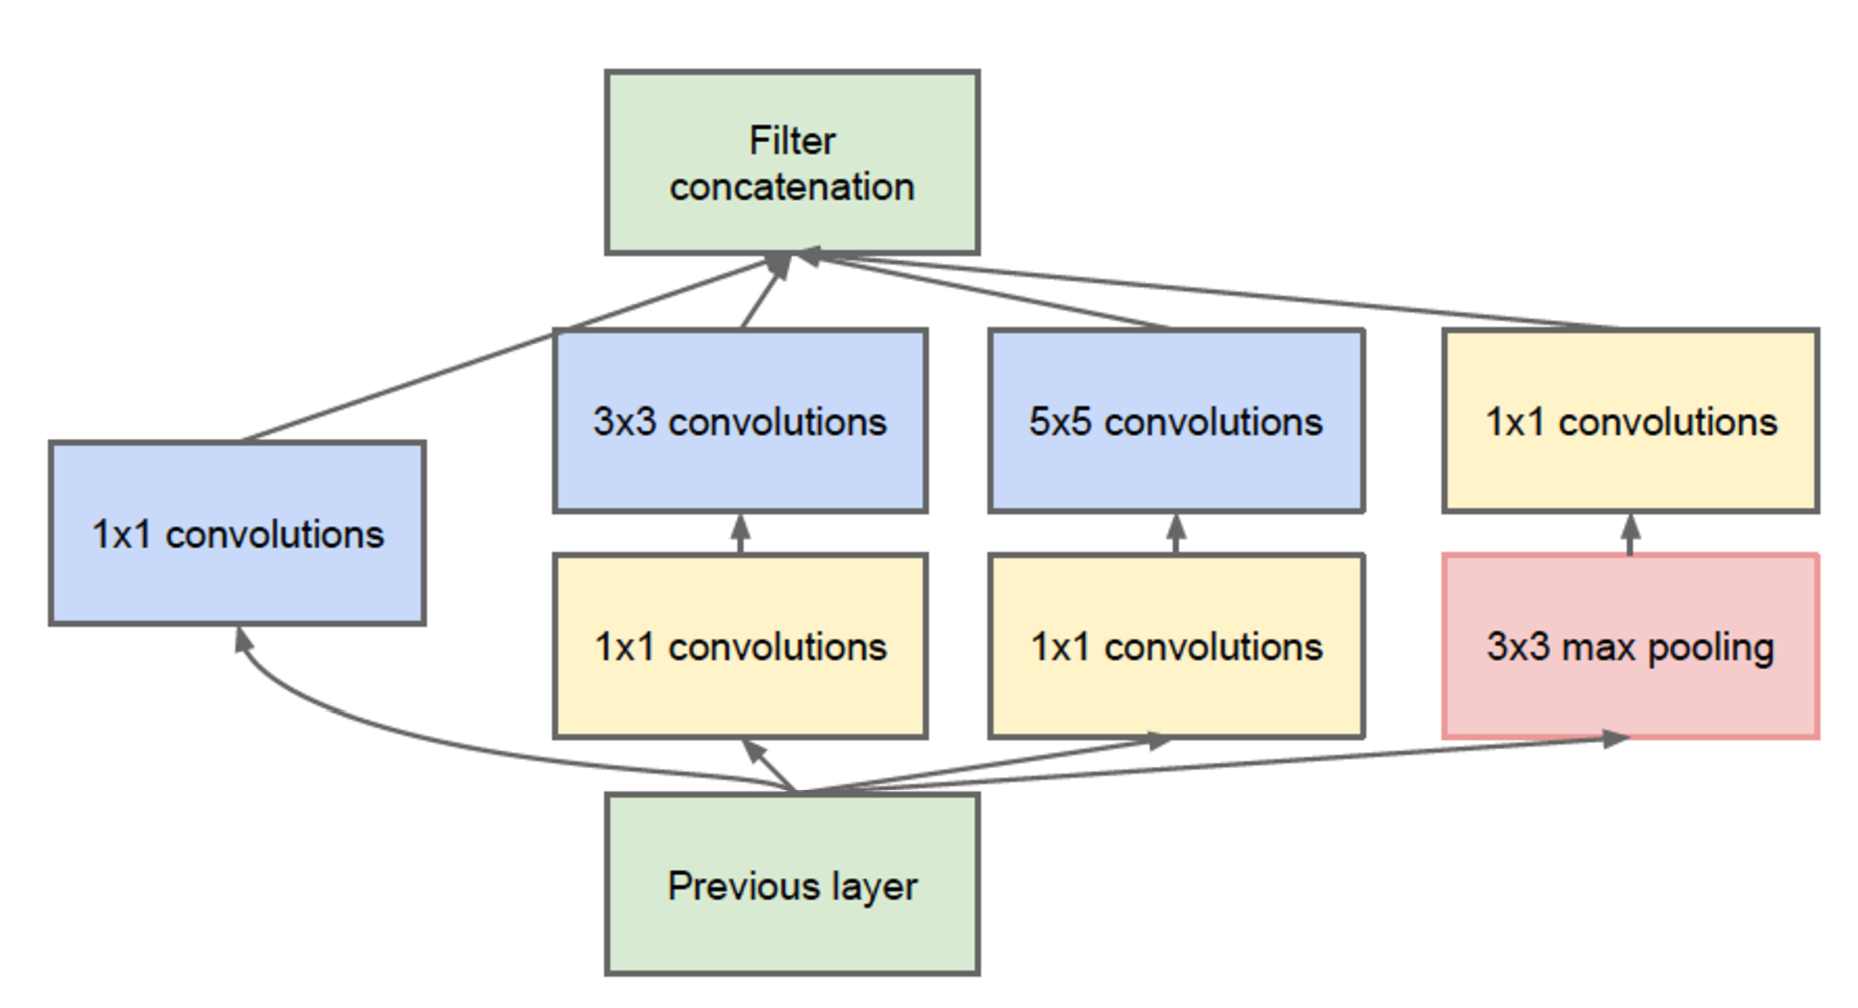
\includegraphics[width =7cm,height=5cm]{Figures/Incb}
\caption{An Inception module.}
\label{InceptionModules}
An Inception module with convolution, max-pooling operations happening in parallel. Here the 1$*$1 convolutions are used  to perform dimensionality reduction.
Image source: Szegedy et al.,2004~\cite{GoogleNet}.
\end{figure}

However, such an implementation could increase the number of parameters in the network and could lead to a \textit{``computational blow up within a few stages''}~\cite{GoogleNet}. In the optimized inception module, $1*1$ convolutions are used to perform dimensionality reductions before the expensive $3*3$ and $5*5$ convolutions. The $1*1$ convolutions reduce the depth of the volume of the output from the previous inception module by performing cross-channel convolutions. The $1*1$ convolutions also help to prevent over-fitting~\cite{NIN}. 

To understand how $1*1$ convolutions work, let us say for example the input to the inception module is $150*150*60$, and applying 20 filters in the $1*1$ convolution block could reduce the volume to $150*150*20$. Then this volume is used as the input to the $3*3$ and $5*5$ convolution blocks. Max-pooling reduces the width and height of the volume whereas 1*1 convolutions minimize the depth of volume. 

In 2015, Szegedy et al. introduced Inception-v2 and Inception-v3 architectures which are slight variants of the original inception modules used in GoogLeNet~\cite{Inception-v3}. In the Inception-v2 and Inception-v3, they introduced factorizations for convolutions greater than $3*3$. For example, a $5*5$ convolution can be replaced by two consecutive layers of 3x3 convolutions and a $7*7$ convolution can be replaced by three consecutive layers of $3*3$ convolutions. Moreover, a $3*3$ convolution could be further broken down into a $3*1$ convolution followed by a $1*3$ convolution which results in a 33\% reduction in computational cost. These factorizations result in different types of inception blocks as summarized in the Figure:~\ref{Inceptiontypes}.

\subsubsection{Residual Networks}

The success of Inception and VGGNet architecture brought us closer to achieving human error at the task of object categorization in the ImageNet dataset. The human top-5 classification error on the ImageNet dataset is 5.1\%~\cite{ImageNETChallenge}. GoogLeNet and VGG16 achieved error rates of 6.7\% and 7.1\% respectively which are very close to the human error. However, the ResNet architectures introduced as a part of the ILSVRC 2015 achieved top 5 error rate of  3.57\% surpassing human error on the task~\cite{ResNet}.


The ResNet or Residual Networks by Kaiming He et al. introduced the concept of residual learning to tackle the problems that arise due to increasing depth of the convolutional neural networks~\cite{ResNet}. The ResNet architecture incorporated techniques such as batch normalization, Skip-connections and use of ReLu as activation function to mitigates the effects of over-fitting and vanishing gradients. The final model which won the ILSVRC 2015 was 152 layers deep with only 60 million parameters compared to VGG19 which had 168 million parameters for 19 layers.

\begin{figure}[t]
\centering
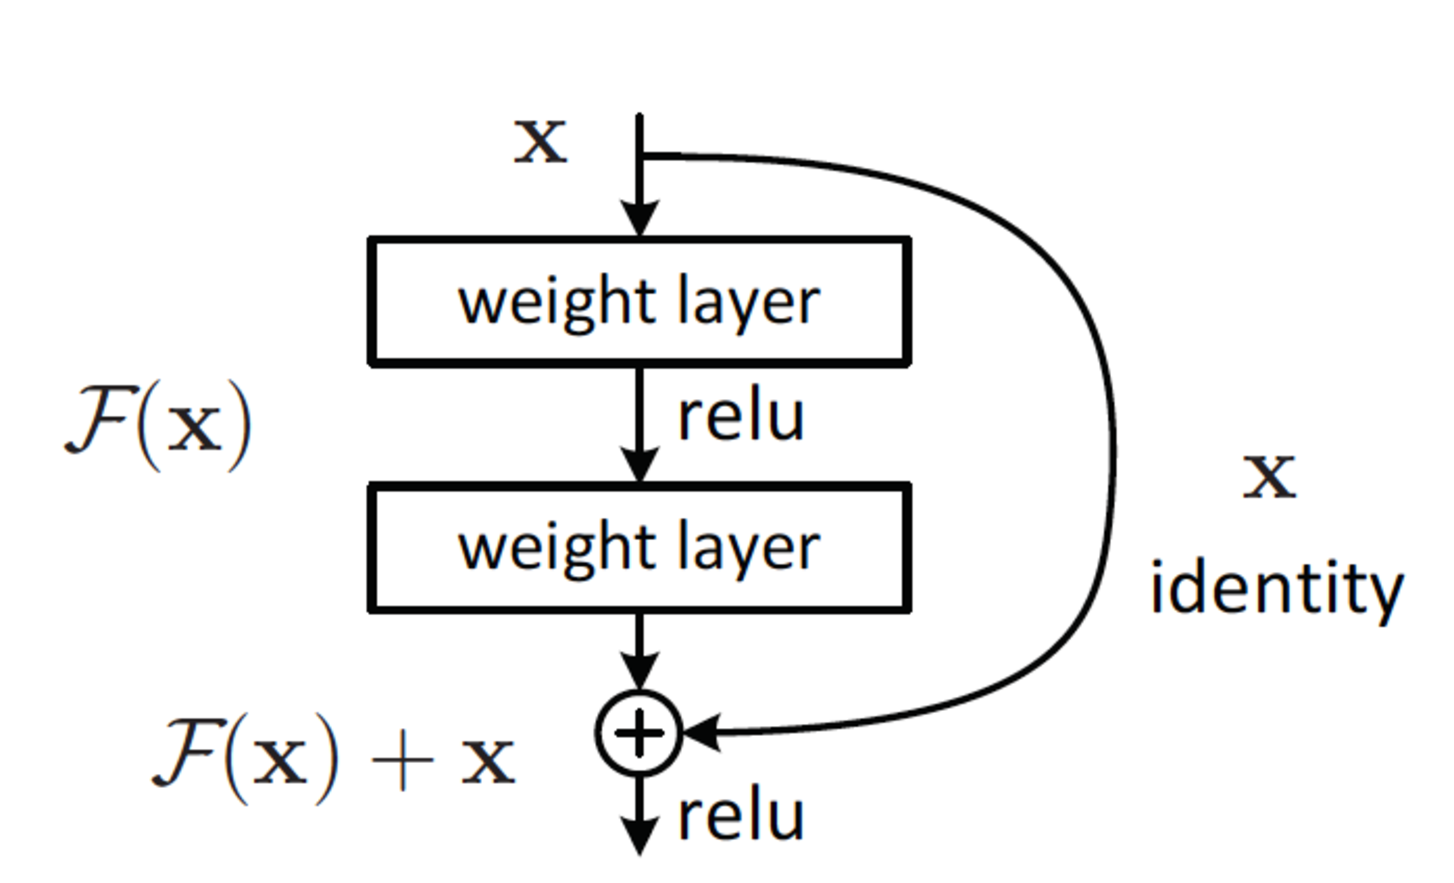
\includegraphics[width=12cm, height=8cm]{Figures/Residual}
\caption{A Residual Learning Block}
\label{ResLearn}
In Residual learning, each identity block tries to learn a small change $F_{(x)}$ and adds it to the input $x$ to get a slightly changed output representation of $H_{(x)}$. \\Image source: Kaiming et al.,2015~\cite{ResNet}
\end{figure}

The principle idea behind the ResNet is the introduction of \textit{``identity short-cut connections''}~\cite{ResNet} that skips through one or more Identity layers in the architecture. An identity layer is a series of convolution layers followed by its activations group together to form one unit. In a simple CNN, an identity layer takes some input $x$ and computes the transformation $H_{(x)}$ which is an entirely new representation of $x$. However, stacking multiple identity layers to form deeper networks is usually associated with a degradation problem. The authors Kaiming et al. argued that instead of computing the direct transformation from $x$ to $H_{(x)}$, we could calculate the term $F_{(x)}$ and add it to the original input $x$ to get $H_{(x)}$~\cite{ResNet}. This means that the identity module is only computing a small change $F_{(x)}$ and adding it to the original input $x$. This is termed as residual learning and is indicated by the Figure:~\ref{ResLearn}

The Residual function is defined as $F_{(x)}=H_{(x)} - x$, where $H_{(x)}$ is the output after a residual operation. To summarize $H_{(x)}$ is learned as $F_{(x)} + x$ which is accomplished by skip-connections between one or more identity blocks in a neural network. Skip-connections were initially introduced as a part of \textit{Highway Networks}~\cite{HighWayNet}. Theoretically, the skip-connections this could allow a large portion of information in the input layers to reach the output layers without degradation. The short-cut connections in residual blocks resemble the ones used in highway networks but does not contain the gated units which act as adaptive mechanism determining if the information should be passed through the short connection or not based on the data. In short, short-cut connections in Residual blocks are data-independent, whereas the ones in highway networks are data-dependent.



ResNets are still considered state of the art and used in the practical applications in computer vision for object recognition tasks. Following ResNet, there were a large number of others networks released combining key architectural elements from ResNet and Inception, but they are beyond the scope of this thesis. Moreover, this work focuses on three main architectures- VGGNet, Inception and ResNet which are quite diverse in their architectural design and also popular among the researchers.

\subsection{Training CNNs}

Training Convolutional Neural Networks is not easy. The labeled dataset is first split into train, validation, and test set. The pixels of the images are then scaled to have mean zero and variance one.  The most important step in the training process is the selection of the learning rate which is initially set at some higher value. The common practice in training deep networks is to reduce the learning rate by half when the learning plateaus (validation loss does not change over a couple of epochs)~\cite{Goodfellow}. During each epoch, we train the CNNs on the training set of images, and validate on the validation set.

Validation set should not be confused with cross-validation. In Convolutional Neural Networks we mostly perform hyperparameter tuning on the validation dataset. The entire data available is divided into training, validation, and test sets. The validation set is used only for hyperparameter tuning, and not used as a part of training. However, in cross-validation, the training data itself is divided into \textit{k} partitions. A machine learning model would be trained on k-1 partitions, and the left out partition is used as validation set. Then, a different partition of the training data could be left out and used for validation. This process is repeated till all the folds are included in the training in the leave-one-out fashion. This process of leaving out a fold, and training on k-1 folds of data is referred to as k-fold cross-validation~\cite{stone1974cross}. Cross-validation method is not recommended for training CNNs due to high computational cost.

Training CNNs often takes many hours or even days. The concept of momentum was introduced to speed up the training process. The main objective of the learning algorithms is to minimize the error (loss) function, and reach the global minimum through repeated iterations of learning. However, in real life scenarios, the error function is not smooth and consists of many local minimum. Sometimes  the algorithm could get stuck at local minimum regions of higher loss. The momentum term increases the step size of the learning iterations of the algorithm and helps the algorithm to converge faster to an ideal local minima of minimal loss.  Momentum also ensures that the gradients move towards the bottom of the bowl shaped error function without much zig-zagging which is generally the case with stochastic gradient descent.

Adaptive learning algorithms such as RMSProp, and Adam~\cite{ADAM} automatically adapts the learning rate based on the gradients calculated during every batch of training. These learning algorithms keep track of gradients calculated over multiple batches, and scales the learning rate for current update. The learning rate is reduced when the gradient is very large and vice versa.

\subsection{Understanding and Visualization of CNN}

CNNs have the potential to change the way machines see our world. However, they are currently black-box, and we don't understand how they come up with their decisions. Their widespread adoption into fields such as diagnostic medicine, space exploration, autonomous driving machines etc. have made them part of our every day human life. Therefore, it becomes essential that we come up with methodologies to unravel the secrets behind their remarkable learning abilities. CNNs designed today have hundreds of hidden layers and millions of parameters, making them even more complex models. The black-box nature of CNNs has been expressed as a major concern by both researchers and early adopters involved in the field of computer vision.


Researchers have adopted several approaches to improve our understanding of convolutional nets. The most common techniques include visualization of activations of the network or visualization of weights, especially in the convolutional layers. Zeiler
et al., 2011 proposed Deconvolutional
Network (Deconv) which approximates the input signal at pixel level by approximating the feature activations in the convolutional blocks~\cite{Deconv}. Zeiler and Fergus used the Deconv net to deconstruct and improve \textit{AlexNet} through visualization of activations for an input image~\cite{ZFNET}. They found properties such as increasing invariance and class discrimination as we moved deeper through the CNN layers. They also occluded parts of images using a mask and studied the class probability predicted by the network. Another simplified approach is to make a small perturbation to the input image such as blurring and to understand the response of the network~\cite{Perturbations}. These techniques help to identify parts of the image that contributes to the classification decisions made by the network.

Another approach is to feed a convolutional net with a large number of images and then identify images which maximally activates a neuron. This helps us to understand and visualize the features that a single neuron might be looking for in its receptive field~\cite{ExciteNeuron}. We could also extract high dimensional feature embeddings from the last hidden layer of a CNN and then use dimensionality reduction techniques such as t-SNE to get a 2-dimensional vector for each image~\cite{t-SNE}. These images can then be plotted on a grid or clustered using unsupervised approaches to visualize them. 

The challenges in the visualization of CNN is mainly due to the fact that most modern architectures have a very large number of neurons, features maps and hidden layers. For each hidden layer, it is possible to study individual neurons, a group of neurons, spatial activations, channel activations or even entire layer (see figure:~\ref{Interpretability}). Therefore, it becomes challenging to bring down the visualization of CNNs to a human-scale. In short, we need to find more efficient and straightforward methods to understand these networks.



\begin{figure}[t]
\centering
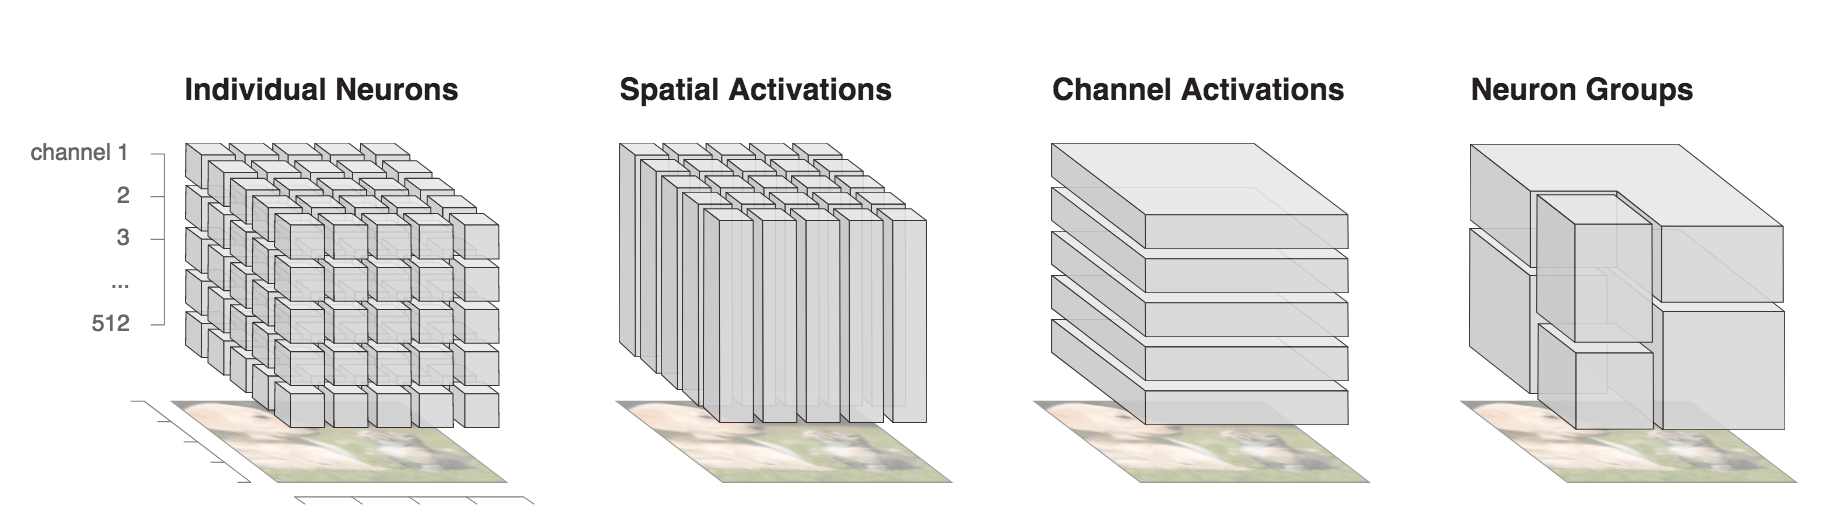
\includegraphics[width=14cm, height=5cm]{Figures/Maps}
\caption{Complexity in CNN Visualizations}
\label{Interpretability}
For each hidden layer in CNN, it is possible to study activations of individual neurons- receptive field of a neuron, spatial activations- spatial positions of certain attributes in an image eg: \textit{wheels of a car}, channel activations- The contribution of a single feature map to the output classifications or even group of neurons- Neurons that activate together for some higher abstract concept\\Image source: Olah et al.,2018  ~\cite{distill2}.
\end{figure}

\subsection{Study of Semantics in CNNs}

Recently there has been some interest among the computer vision community to study semantic representations instead of the internal feature representations in CNN. Gonzalez-Garcia et al., 2017~\cite{SemanticCNN} studied emergence of semantics in \textit{AlexNet} using PASCAL-Part dataset~\cite{Pascal_part}. The PASCAL-Part dataset is a subset of PASCAL VOC, 2010 dataset~\cite{pascal-voc-2010} with bounding boxes separating semantic areas in images. They created visualizations for filter activations in the L-5 layer of AlexNet (256 filters) for 16 object classes. The human annotators were asked to label all the 256 filter activations as \textit{semantic part or not} for every object category. They found that filter activations corresponding to semantic areas only contributed to 7\% of the total filter activations. 


However, studying semantics of a particular layer of a network may not offer us more insights as compared to studying the growth of semantic representation as a function of depth of the network. Moreover, use of human annotators to label and identify filter activations corresponding to semantics parts of an image is not feasible for larger networks. The process could become tedious and time-consuming. PASCAL VOC, 2010 dataset has only 20 object classes compared to 1000 classes in ImageNet. This further strengthens our argument about the need for a simple and efficient method to study semantic representation in CNN.

Computational models such as Convolutional Neural Networks could also be used to study visual feature representation in the human brain. Visual features extracted from CNNs have been shown to correlate with fMRI patterns of participants viewing visuals of objects~\cite{BrainCNN3}. The features extracted from these models have also been able to predict fMRI activities of unseen object classes (Concept class the CNN was not trained initially to predict). Another work by Wen et al., 2017 could predict fMRI activities corresponding to humans watching movies using features extracted from ConvNet layers~\cite{BrainCNN2}. This is despite the fact that fMRI does not capture any temporal properties of brain activations.

Cichy et al., 2016 found similarities between voxel-level activations in dorsal and ventral regions in the human brain and the hierarchical features extracted from layers of CNN using fMRI and MEG data~\cite{BrainCNN1}. The authors concluded that initial layers of CNN showed similarities to the occipital lobe (low and mid-level visual region) and for deeper layers of CNN, the similarities corresponded to the dorsal and ventral regions in the anterior brain. In short, layers of these networks could be mapped back to regions in the human brain.

Despite all these remarkable results, brain data is prohibitively expensive and time consuming to collect, process and analyze. Most of the studies comparing CNN to brain explored simple networks such as AlexNet (just eight layers) as compared to deeper networks such as ResNet or VGGNet. Moreover, those studies incorporated very few coarse concepts (usually up to 20 concepts classes) compared to 1000 classes in ImageNet that includes fine-grained concepts such as different species of dogs for a single coarse concept class \textit{dog}. These limitations reiterate the need for a simple methodology to study semantic representations in CNN. 

This thesis proposes to use Distributional Semantic models such as Skip-Gram, Glove etc. that are trained on text corpora to study the convergence of semantic representations through the depth of a CNN architecture. These DS models usually have ample coverage for concepts in ImageNet and are available as pre-trained text files. Moreover, our methodology described in \textit{Chapter 4} generalize very well to study CNN architectures of varying complexity and depth. We also present the details of our experiments with three diverse networks (VGGNet, Inception-v3 and ResNet) in our \textit{Chapter 4}.

\section{Summary}

This chapter discussed in detail about related works in the field of Computational Linguistics focused towards the study of semantics in brain, text and images. We introduced Distributional Semantic models trained on text corpora and discussed some of the most popular DS models. A discussion on various methods to evaluate and benchmark word vectors was done. We then discussed in brief about convolutional neural networks and problems associated with their black-box nature. Some of the existing methods to study CNN architectures were also discussed in this chapter. In the next chapter, we discuss in detail on BrainBench, highlighting our contributions toward improving the tool along with results and discussions on our experiments with various brain datasets.







